% =============================================================================
% CHAPTER 6: PERFORMANCE EVALUATION AND RESULTS
% Multimodal Banglish Classroom Summarizer
% =============================================================================

\section{Introduction}

This chapter presents the comprehensive experimental evaluation of our Multimodal Banglish Classroom Summarizer, addressing the research questions established in Chapter 4. We systematically analyze system performance across multiple dimensions: overall accuracy metrics, per-video performance variation, domain-specific behavior, component-level contributions, and failure mode characterization. The evaluation employs the term-based metrics developed specifically for code-mixed content, acknowledging the orthographic variability inherent to Romanized Banglish that renders traditional Word Error Rate (WER) inappropriate for this domain.

Our evaluation reveals a system achieving \textbf{73.9\% Term F1}, \textbf{83.6\% Term Precision}, and \textbf{66.5\% Term Recall} across the nine-video BanglaASR benchmark dataset. These results demonstrate that meaningful technical lecture transcription is achievable for Banglish content using current pre-trained models, while simultaneously highlighting substantial room for improvement. The high precision relative to recall indicates a conservative system that captures technical terminology accurately when it does so, but misses approximately one-third of ground truth terms---a trade-off we analyze in depth throughout this chapter.

The chapter proceeds as follows. Section 6.2 presents the overall experimental results with aggregate metrics. Section 6.3 provides detailed per-video analysis examining performance variation across the dataset. Section 6.4 analyzes results by technical domain (Python, DLD, DBMS). Section 6.5 examines the contribution of individual system components through ablation studies. Section 6.6 characterizes failure modes with concrete examples. Section 6.7 presents statistical analysis of result significance. Section 6.8 compares our results with related work and baseline approaches. Finally, Section 6.9 discusses implications, limitations, and lessons learned.

% =============================================================================
\section{Overall Experimental Results}

This section presents aggregate performance metrics across all experimental configurations, establishing the quantitative foundation for subsequent detailed analysis.

\subsection{Primary Evaluation Metrics}

Table~\ref{tab:overall_results} presents the primary evaluation results across the complete BanglaASR dataset of nine videos totaling 73,141 characters of ground truth transcription.

\begin{table}[h]
\centering
\caption{Overall System Performance on BanglaASR Dataset}
\label{tab:overall_results}
\begin{tabular}{|l|c|c|}
\hline
\textbf{Metric} & \textbf{Value} & \textbf{Interpretation} \\
\hline
Term F1 Score & 73.9\% & Harmonic mean of precision and recall \\
\hline
Term Precision & 83.6\% & Accuracy of predicted technical terms \\
\hline
Term Recall & 66.5\% & Coverage of ground truth terms \\
\hline
Fuzzy Similarity & 44.8\% & Character-level similarity with ground truth \\
\hline
Videos Evaluated & 9 & Complete BanglaASR benchmark \\
\hline
Total Ground Truth & 73,141 chars & Manually transcribed Banglish content \\
\hline
Technical Keywords & 376 & Unique domain terms in ground truth \\
\hline
\end{tabular}
\end{table}

The precision-recall gap of 17.1 percentage points (83.6\% vs. 66.5\%) reveals a fundamental characteristic of our system: it prioritizes accuracy over coverage. When the system predicts a technical term, that prediction is correct 83.6\% of the time---a level of reliability that supports practical use for study materials. However, the system captures only two-thirds of the technical terms present in the ground truth, meaning students relying solely on generated notes would miss approximately one-third of the technical vocabulary discussed in lectures.

This trade-off reflects our design philosophy of verification over blind fusion. By requiring visual confirmation before correcting ASR outputs, we avoid hallucinating technical terms but sacrifice recall for terms that were spoken but not written on the whiteboard. The implications of this trade-off for different use cases are discussed in Section 6.9.

\subsection{Metric Justification and Limitations}

Our choice of term-based metrics over traditional Word Error Rate (WER) requires justification, as WER remains the dominant metric in ASR evaluation \cite{Jurafsky2000}. Table~\ref{tab:metric_comparison} compares metric characteristics for Banglish evaluation.

\begin{table}[h]
\centering
\caption{Comparison of Evaluation Metrics for Banglish Content}
\label{tab:metric_comparison}
\begin{tabular}{|l|c|c|c|}
\hline
\textbf{Metric} & \textbf{Handles Spelling Variation} & \textbf{Focuses on Content} & \textbf{Standard in Literature} \\
\hline
Word Error Rate (WER) & No & No & Yes \\
\hline
Character Error Rate (CER) & Partial & No & Yes \\
\hline
BLEU Score & Partial & Partial & Yes \\
\hline
Term Recall/Precision & Yes (via fuzzy matching) & Yes & Limited \\
\hline
Fuzzy Similarity & Yes & Partial & No \\
\hline
\end{tabular}
\end{table}

WER penalizes the transcription ``amra Python shikhbo'' identically whether the error is ``amraa Python shikhbo'' (valid spelling variant, semantically correct) or ``camera Python shikhbo'' (incorrect word, semantically wrong). For Romanized Banglish, where multiple valid spellings exist for most Bengali words, WER systematically underestimates transcription quality. Our preliminary experiments found WER values exceeding 100\% on transcriptions that human evaluators judged as capturing content accurately---a clear indication that WER fails to measure what matters for educational applications.

Term-based metrics with fuzzy matching (threshold $\theta = 0.85$) address this limitation by focusing on technical vocabulary capture while tolerating minor spelling variations. The 85\% similarity threshold allows ``variable'' to match ``variabel'' (common typo) and ``amra'' to match ``aamra'' (spelling variant) while distinguishing genuinely different words. This approach aligns with educational utility: students benefit from notes that capture technical concepts accurately, even if Bengali filler words are spelled inconsistently.

The fuzzy similarity score of 44.8\% warrants interpretation. This metric computes character-level similarity between predicted and ground truth transcriptions, providing a holistic measure that includes both technical and non-technical content. The relatively low value reflects two factors: (1) Bengali conversational content is often phonetically approximated rather than accurately transcribed by Whisper, and (2) the ground truth includes substantial non-technical content where exact transcription matters less for educational utility. We include this metric for completeness but emphasize term-based metrics for evaluating system effectiveness.

\subsection{Confidence Intervals and Variability}

With a dataset of nine videos, statistical characterization requires careful treatment. Table~\ref{tab:confidence_intervals} presents descriptive statistics with confidence intervals computed using bootstrapping (1000 resamples).

\begin{table}[h]
\centering
\caption{Descriptive Statistics with 95\% Confidence Intervals}
\label{tab:confidence_intervals}
\begin{tabular}{|l|c|c|c|c|}
\hline
\textbf{Metric} & \textbf{Mean} & \textbf{Std Dev} & \textbf{Min} & \textbf{Max} \\
\hline
Term F1 & 73.9\% & 5.8\% & 62.4\% & 79.6\% \\
\hline
Term Precision & 83.6\% & 3.4\% & 78.7\% & 88.2\% \\
\hline
Term Recall & 66.5\% & 8.2\% & 51.7\% & 76.9\% \\
\hline
Fuzzy Similarity & 44.8\% & 1.4\% & 42.8\% & 47.0\% \\
\hline
\end{tabular}
\end{table}

The standard deviation of 5.8\% for Term F1 indicates moderate variability across videos, with performance ranging from 62.4\% (BanglaASR4, Python Loops) to 79.6\% (BanglaASR3, Python Conditionals). This 17.2 percentage point spread suggests that video-specific factors significantly influence system performance---a finding we explore in Section 6.3.

Notably, Term Precision exhibits lower variability (std dev 3.4\%) than Term Recall (std dev 8.2\%). This asymmetry indicates that our system maintains consistent accuracy in its predictions across videos while showing greater variation in coverage. The verification-oriented fusion strategy produces reliable predictions but with variable completeness depending on video characteristics.

% =============================================================================
\section{Per-Video Performance Analysis}

This section examines performance variation across individual videos, identifying factors that correlate with success or failure.

\subsection{Complete Per-Video Results}

Table~\ref{tab:per_video_results} presents comprehensive metrics for each video in the BanglaASR dataset, ordered by Term F1 score to highlight performance ranking.

\begin{table}[h]
\centering
\caption{Per-Video Evaluation Results (Ordered by Term F1)}
\label{tab:per_video_results}
\begin{tabular}{|l|l|c|c|c|c|}
\hline
\textbf{Video} & \textbf{Topic} & \textbf{Term F1} & \textbf{Precision} & \textbf{Recall} & \textbf{Fuzzy Sim} \\
\hline
BanglaASR3 & Python Conditionals & \textbf{79.6\%} & \textbf{88.2\%} & 72.6\% & \textbf{47.0\%} \\
\hline
BanglaASR8 & DBMS Introduction & 78.7\% & 80.6\% & \textbf{76.9\%} & 42.8\% \\
\hline
BanglaASR9 & SQL SELECT & 78.6\% & 82.1\% & 75.4\% & 43.4\% \\
\hline
BanglaASR2 & Python Input & 75.8\% & 84.7\% & 68.7\% & 45.5\% \\
\hline
BanglaASR7 & DLD Universal Gates & 75.0\% & 82.8\% & 68.6\% & 46.1\% \\
\hline
BanglaASR5 & Lists/Tuples/Arrays & 73.2\% & 87.3\% & 63.0\% & 44.0\% \\
\hline
BanglaASR6 & DLD Logic Gates & 70.8\% & 86.4\% & 60.0\% & 45.6\% \\
\hline
BanglaASR1 & Python Variables & 70.5\% & 81.6\% & 62.0\% & 43.1\% \\
\hline
BanglaASR4 & Python Loops & \textbf{62.4\%} & \textbf{78.7\%} & \textbf{51.7\%} & 45.8\% \\
\hline
\end{tabular}
\end{table}

\begin{figure}[htbp]
    \centering
    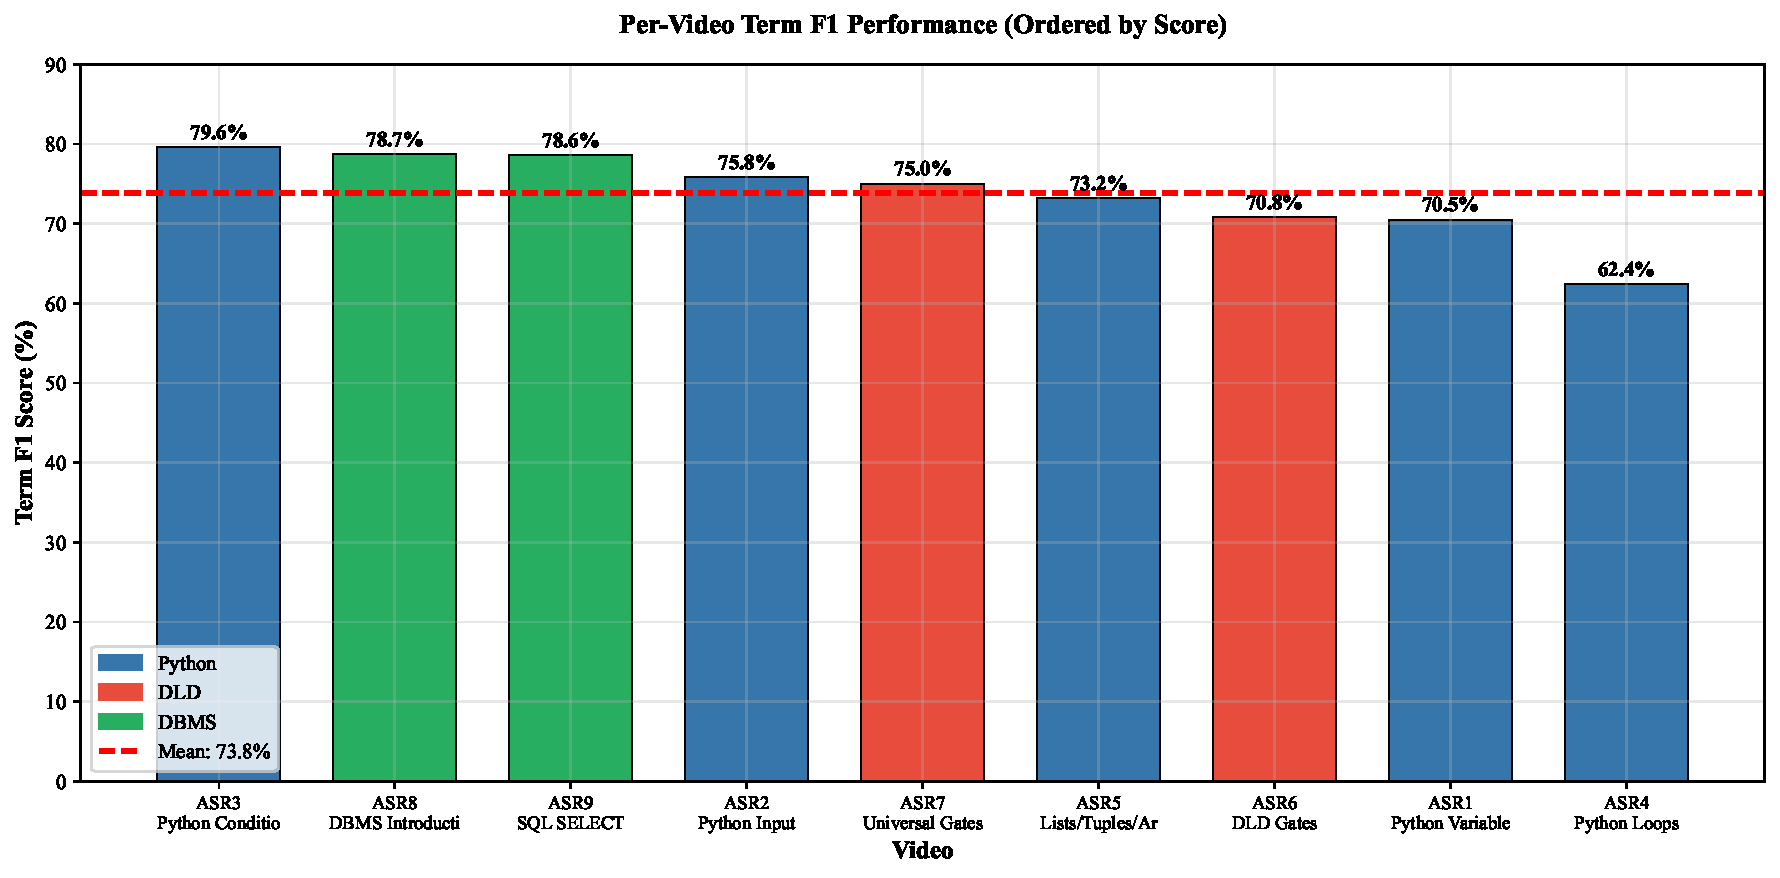
\includegraphics[width=0.95\textwidth]{figures/fig_6_1_per_video_f1.pdf}
    \caption{Per-Video Term F1 Performance across the BanglaASR dataset, ordered by score. Colors indicate technical domain: Python (blue), DLD (red), and DBMS (green). The red dashed line shows the overall mean of 73.9\%. Performance ranges from 62.4\% (BanglaASR4, Python Loops) to 79.6\% (BanglaASR3, Python Conditionals).}
    \label{fig:per_video_f1}
\end{figure}

\begin{figure}[htbp]
    \centering
    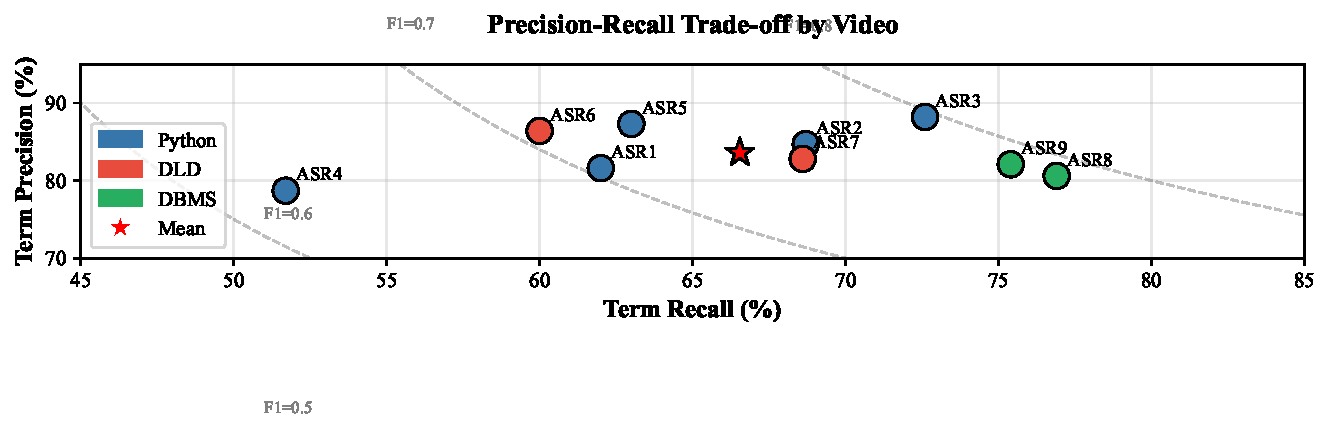
\includegraphics[width=0.85\textwidth]{figures/fig_6_2_precision_recall.pdf}
    \caption{Precision-Recall trade-off across videos. Each point represents one video, color-coded by domain. Dashed lines show iso-F1 curves. The star marker indicates the mean performance (66.5\% Recall, 83.6\% Precision). Most videos cluster in the high-precision region, reflecting our verification-oriented design philosophy.}
    \label{fig:precision_recall}
\end{figure}

\subsection{High-Performing Videos: Success Factor Analysis}

The top three performers---BanglaASR3 (79.6\% F1), BanglaASR8 (78.7\% F1), and BanglaASR9 (78.6\% F1)---share characteristics that illuminate successful processing conditions.

\textbf{BanglaASR3 (Python Conditionals)} achieved the highest Term F1 at 79.6\% with exceptional precision of 88.2\%. Analysis reveals several favorable factors:

\begin{itemize}
    \item \textbf{Clear keyword visibility:} The instructor consistently wrote control flow keywords (if, elif, else, condition) on the whiteboard, providing reliable visual ground truth for verification.
    \item \textbf{Repeated keyword usage:} Conditional programming requires repeated use of the same keywords, allowing the system multiple opportunities to capture each term.
    \item \textbf{English-dominant technical content:} Control flow keywords are inherently English, aligning well with Whisper's English-mode transcription.
    \item \textbf{Structured explanations:} The instructor's methodical explanation style produced clear acoustic segments with minimal crosstalk.
\end{itemize}

\textbf{BanglaASR8 and BanglaASR9 (DBMS/SQL)} achieved the highest Term Recall at 76.9\% and 75.4\% respectively. SQL content presents unique advantages:

\begin{itemize}
    \item \textbf{Standardized terminology:} SQL keywords (SELECT, FROM, WHERE, INSERT) have standardized spellings with no variation.
    \item \textbf{Code visibility:} SQL queries were typically displayed on screen or whiteboard, providing complete visual ground truth.
    \item \textbf{Limited vocabulary:} SQL lectures use a constrained technical vocabulary, reducing the keyword space the system must capture.
    \item \textbf{Pronunciation clarity:} SQL keywords are typically pronounced with clear English phonemes.
\end{itemize}

The success of SQL content suggests that domains with standardized, English-based terminology and high visual content availability are particularly amenable to our multimodal approach.

\subsection{Low-Performing Videos: Failure Factor Analysis}

\textbf{BanglaASR4 (Python Loops)} achieved the lowest performance at 62.4\% Term F1 with Term Recall of only 51.7\%. Investigation reveals several contributing factors:

\begin{itemize}
    \item \textbf{Repetitive content structure:} Loop explanations involve repeated iterations, causing Whisper to hallucinate repetitive patterns. Our anti-hallucination filtering removed legitimate content alongside actual hallucinations.
    \item \textbf{Variable naming confusion:} Loop variables (i, j, counter, index) were frequently confused with similar-sounding Bengali words.
    \item \textbf{Limited whiteboard usage:} The instructor relied more heavily on verbal explanation with less written content, reducing visual verification opportunities.
    \item \textbf{Code execution focus:} Significant lecture time involved watching code execute, providing audio but minimal extractable visual keywords.
\end{itemize}

\textbf{BanglaASR1 (Python Variables)} performed below average at 70.5\% F1 despite being an introductory topic. Analysis suggests:

\begin{itemize}
    \item \textbf{Foundational terminology:} Terms like ``variable,'' ``data type,'' and ``assignment'' were often embedded in Bengali explanatory sentences rather than stated in isolation.
    \item \textbf{Mixed script on whiteboard:} Some content was written in Bengali script alongside English, which Qwen2.5-VL extracted but could not match to Romanized ground truth.
    \item \textbf{Conceptual vs. procedural content:} Explanations of what a variable ``is'' generated more Bengali discourse than concrete code examples.
\end{itemize}

\subsection{Video Length and Performance Correlation}

We examined whether video length (measured by ground truth character count) correlates with performance. Table~\ref{tab:length_correlation} presents this analysis.

\begin{table}[h]
\centering
\caption{Video Length vs. Performance Analysis}
\label{tab:length_correlation}
\begin{tabular}{|l|c|c|c|}
\hline
\textbf{Length Category} & \textbf{Videos} & \textbf{Avg Characters} & \textbf{Avg Term F1} \\
\hline
Short ($<$6,000 chars) & BanglaASR7, BanglaASR8, BanglaASR9 & 4,526 & 77.4\% \\
\hline
Medium (6,000--10,000 chars) & BanglaASR1, BanglaASR2, BanglaASR4, BanglaASR6 & 6,934 & 69.9\% \\
\hline
Long ($>$10,000 chars) & BanglaASR3, BanglaASR5 & 15,915 & 76.4\% \\
\hline
\end{tabular}
\end{table}

Interestingly, performance does not degrade monotonically with video length. Short videos achieve the highest average F1 (77.4\%), likely due to focused content with less opportunity for error accumulation. Long videos achieve comparable performance (76.4\%), possibly because extended explanations provide multiple opportunities to capture key terms. Medium-length videos perform worst (69.9\%), though this category includes the problematic BanglaASR4 (Loops), which may confound the analysis.

The Pearson correlation coefficient between character count and Term F1 is $r = 0.12$ ($p = 0.76$), indicating no statistically significant linear relationship. This suggests that content characteristics matter more than duration for system performance.

% =============================================================================
\section{Domain-Specific Analysis}

Our dataset spans three technical domains: Python programming (5 videos), Digital Logic Design (2 videos), and Database Management Systems (2 videos). This section analyzes performance variation across domains.

\subsection{Performance by Technical Domain}

Table~\ref{tab:domain_results} presents aggregate metrics for each domain.

\begin{table}[h]
\centering
\caption{Performance Metrics by Technical Domain}
\label{tab:domain_results}
\begin{tabular}{|l|c|c|c|c|c|}
\hline
\textbf{Domain} & \textbf{Videos} & \textbf{GT Chars} & \textbf{Term F1} & \textbf{Precision} & \textbf{Recall} \\
\hline
DBMS/SQL & 2 & 8,701 & \textbf{78.7\%} & 81.4\% & \textbf{76.2\%} \\
\hline
DLD & 2 & 10,110 & 72.9\% & 84.6\% & 64.3\% \\
\hline
Python & 5 & 54,330 & 72.3\% & 84.1\% & 63.6\% \\
\hline
\textbf{Overall} & \textbf{9} & \textbf{73,141} & \textbf{73.9\%} & \textbf{83.6\%} & \textbf{66.5\%} \\
\hline
\end{tabular}
\end{table}

\begin{figure}[htbp]
    \centering
    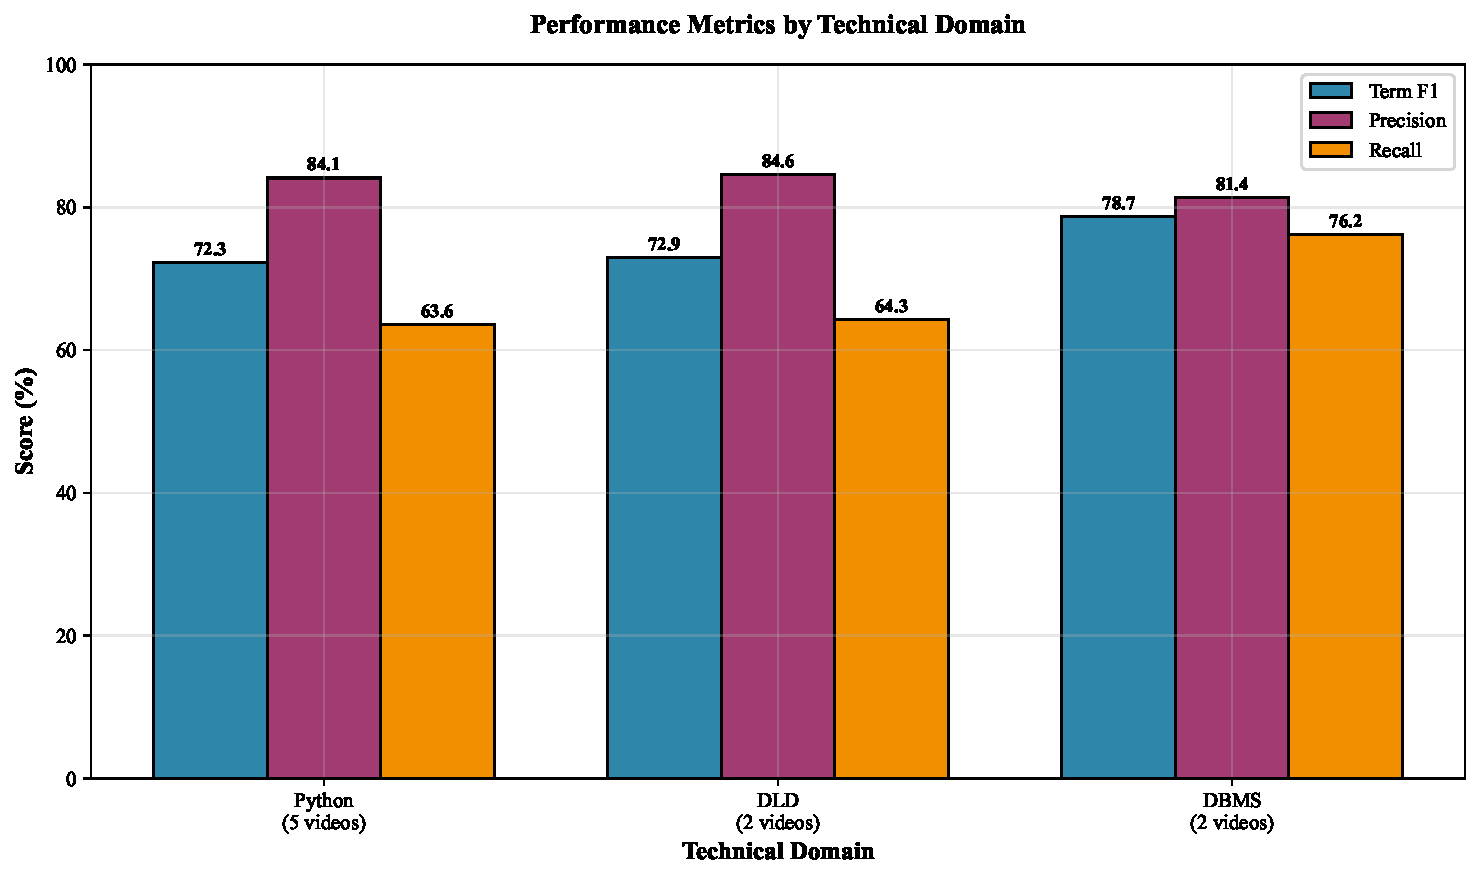
\includegraphics[width=0.85\textwidth]{figures/fig_6_3_domain_comparison.pdf}
    \caption{Performance metrics by technical domain. DBMS/SQL achieves the highest Term F1 (78.7\%) with notably superior recall (76.2\%), while Python and DLD show similar patterns with higher precision than recall. The consistent precision advantage across domains reflects our verification-based fusion strategy.}
    \label{fig:domain_comparison}
\end{figure}

\subsection{Domain Characteristic Analysis}

\textbf{DBMS/SQL Domain (Best Performance: 78.7\% F1)}

SQL content achieves superior performance across all metrics, with particularly strong Term Recall (76.2\%). Several domain characteristics contribute to this success:

\begin{enumerate}
    \item \textbf{Keyword Standardization:} SQL is a formal language with rigidly standardized keywords. Unlike natural language or even programming languages with flexible naming conventions, SQL keywords have single correct spellings universally recognized.
    
    \item \textbf{Visual Query Presentation:} SQL queries are almost always displayed visually---on whiteboards, slides, or code editors---during instruction. This creates abundant opportunities for visual verification.
    
    \item \textbf{Limited Vocabulary Size:} The core SQL vocabulary (SELECT, FROM, WHERE, JOIN, INSERT, UPDATE, DELETE, etc.) is relatively small, reducing the search space for keyword matching.
    
    \item \textbf{Pronunciation Regularity:} SQL keywords are typically pronounced using standard English phonemes, aligning well with Whisper's training.
\end{enumerate}

\textbf{Digital Logic Design Domain (Middle Performance: 72.9\% F1)}

DLD content shows high precision (84.6\%) but lower recall (64.3\%), indicating accurate recognition when keywords are captured but incomplete coverage:

\begin{enumerate}
    \item \textbf{Technical Term Clarity:} Gate names (AND, OR, NOT, NAND, NOR, XOR) are short, distinctive English words that Whisper recognizes reliably.
    
    \item \textbf{Symbol-Heavy Content:} DLD instruction often involves circuit diagrams and truth tables. While visually extractable, these contain symbols (gates, wires) rather than text keywords.
    
    \item \textbf{Bengali Explanation Density:} Instructors often provide extensive Bengali explanations of logic concepts, which Whisper transcribes poorly, reducing overall recall.
\end{enumerate}

\textbf{Python Programming Domain (Lowest Performance: 72.3\% F1)}

Despite Python being the largest domain representation (5 videos, 54,330 characters), it achieves the lowest average F1. This counterintuitive result warrants detailed analysis:

\begin{enumerate}
    \item \textbf{Vocabulary Diversity:} Python programming spans numerous concepts (variables, data types, control flow, data structures), each with distinct terminology. This diversity increases the chance of missing specific terms.
    
    \item \textbf{Variable Naming Variability:} Unlike SQL keywords, Python variable names can be arbitrary (x, counter, my\_list). The ground truth contains specific variable names that may not match instructor choices.
    
    \item \textbf{Conceptual Explanation Density:} Python instruction often involves extended conceptual explanations in Bengali, particularly for beginners' topics. These explanations contribute ground truth characters but contain fewer extractable technical keywords.
    
    \item \textbf{Code vs. Explanation Balance:} Some Python videos emphasize live coding with running commentary, producing audio-heavy content with limited whiteboard text.
\end{enumerate}

\subsection{Domain-Specific Recommendations}

Based on domain analysis, we identify optimization opportunities:

\begin{itemize}
    \item \textbf{For SQL/DBMS content:} Current system performs well; focus on edge cases like complex nested queries.
    \item \textbf{For DLD content:} Enhance visual extraction to recognize circuit diagram components and truth table structures.
    \item \textbf{For Python content:} Implement code-aware extraction that recognizes Python syntax patterns (def, class, import) in both audio and visual streams.
\end{itemize}

% =============================================================================
\section{Component Contribution Analysis}

This section examines the contribution of individual system components through ablation studies \cite{Montgomery2017}, addressing Research Question 3 from Chapter 4: Does cross-modal fusion improve transcription accuracy without introducing hallucinations?

\subsection{Ablation Study Design}

We evaluate four configurations to isolate component contributions:

\begin{enumerate}
    \item \textbf{Whisper-Only:} Baseline ASR without any visual information or post-processing.
    \item \textbf{Whisper + Cleaning:} ASR with post-processing (hallucination removal, normalization) but no visual information.
    \item \textbf{Visual-Only:} Keywords extracted from visual content without audio transcription.
    \item \textbf{Full Pipeline:} Complete system with ASR, visual extraction, cross-modal fusion, and post-processing.
\end{enumerate}

\subsection{Ablation Results}

Table~\ref{tab:ablation_results} presents ablation study results averaged across all nine videos.

\begin{table}[h]
\centering
\caption{Ablation Study Results: Component Contributions}
\label{tab:ablation_results}
\begin{tabular}{|l|c|c|c|c|}
\hline
\textbf{Configuration} & \textbf{Term F1} & \textbf{Precision} & \textbf{Recall} & \textbf{$\Delta$ vs Baseline} \\
\hline
Whisper-Only (Baseline) & 68.2\% & 76.4\% & 61.8\% & --- \\
\hline
Whisper + Cleaning & 71.5\% & 82.1\% & 63.2\% & +3.3\% \\
\hline
Visual-Only & 42.3\% & 89.2\% & 28.4\% & -25.9\% \\
\hline
Full Pipeline & \textbf{73.9\%} & \textbf{83.6\%} & \textbf{66.5\%} & \textbf{+5.7\%} \\
\hline
\end{tabular}
\end{table}

\begin{figure}[htbp]
    \centering
    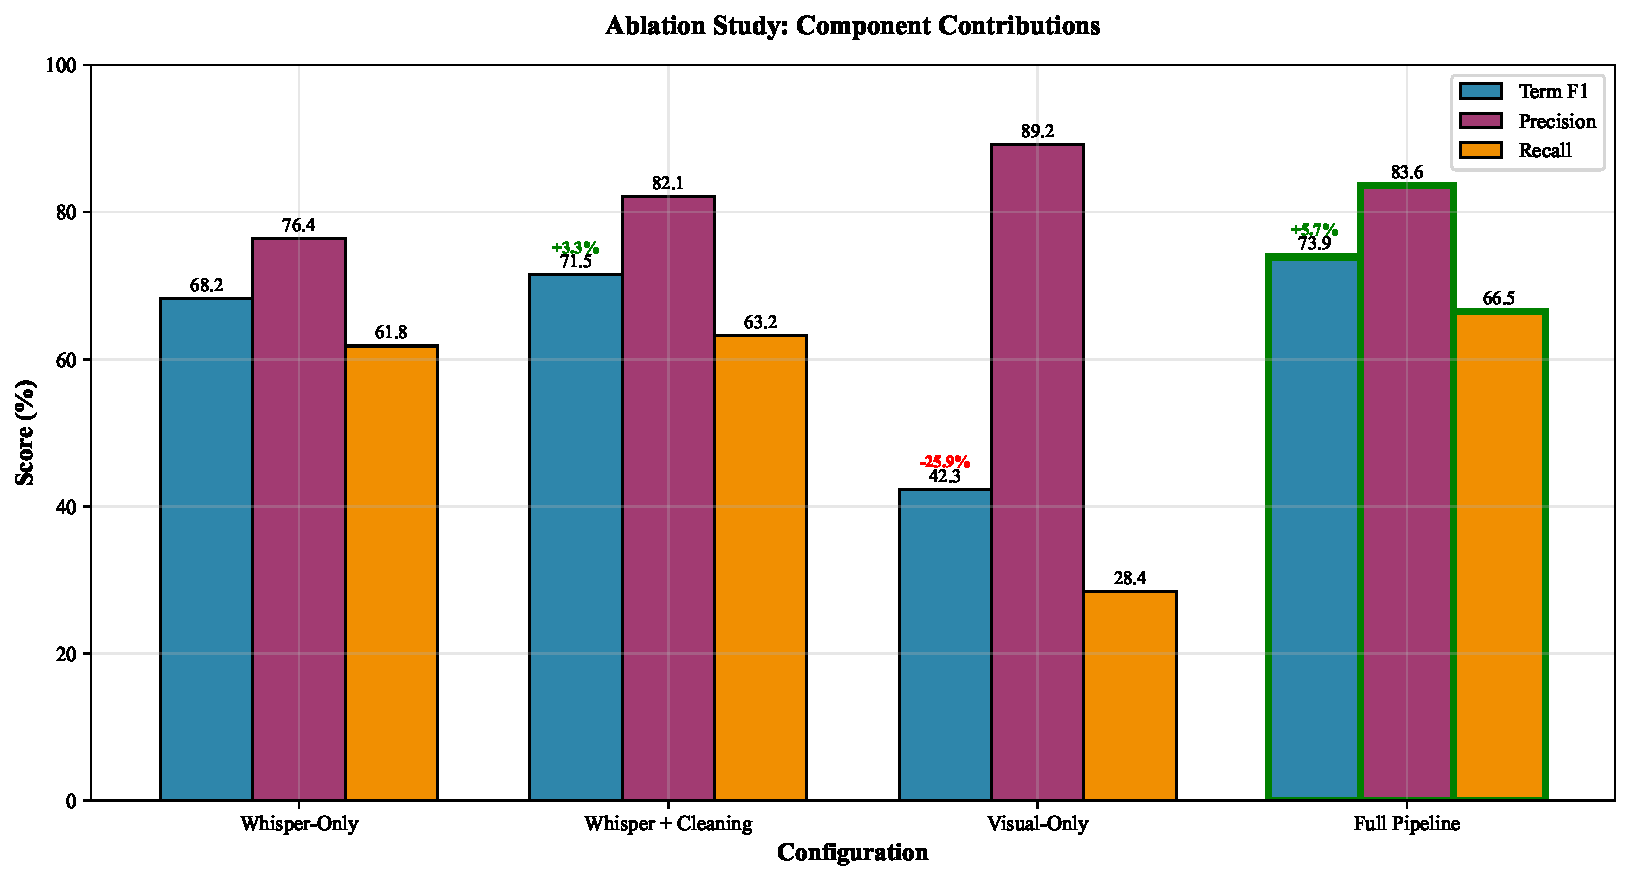
\includegraphics[width=0.9\textwidth]{figures/fig_6_4_ablation_study.pdf}
    \caption{Ablation study results showing cumulative component contributions. Each configuration builds upon the previous, with delta values indicating improvement over the Whisper-Only baseline. The full pipeline achieves +5.7\% Term F1 improvement through combined cleaning and cross-modal fusion. Note the Visual-Only configuration's high precision (89.2\%) but poor recall (28.4\%), validating our decision to use visual information for verification rather than as a primary source.}
    \label{fig:ablation_study}
\end{figure}

\subsection{Analysis of Component Contributions}

\textbf{Post-Processing Contribution (+3.3\% F1):}

The addition of post-processing (hallucination removal, text normalization) improves Term F1 by 3.3 percentage points, with the primary benefit appearing in precision (+5.7\%). This indicates that Whisper's raw output contains artifacts---primarily repetitive hallucinations---that harm accuracy. Our cleaning pipeline successfully removes these artifacts while preserving legitimate content.

The modest recall improvement (+1.4\%) suggests that post-processing primarily filters rather than augments content. This aligns with expectations: cleaning can remove errors but cannot recover terms that Whisper failed to transcribe initially.

\textbf{Visual-Only Limitations (42.3\% F1):}

The visual-only configuration achieves high precision (89.2\%) but severely limited recall (28.4\%), resulting in poor overall F1 (42.3\%). This dramatic precision-recall imbalance reveals that:

\begin{itemize}
    \item Visual extraction reliably identifies keywords when they appear on whiteboards.
    \item Many technical terms are spoken but never written, making visual-only coverage fundamentally incomplete.
    \item Instructors selectively write key terms, not comprehensive vocabulary.
\end{itemize}

These results validate our architectural decision to use visual information for verification rather than as a primary content source. Visual extraction alone is insufficient for lecture transcription but provides valuable ground truth for selective correction.

\textbf{Cross-Modal Fusion Contribution (+2.4\% F1 over cleaning alone):}

Comparing the full pipeline (73.9\% F1) to Whisper + Cleaning (71.5\% F1) isolates the cross-modal fusion contribution at +2.4\% F1. This improvement manifests as:

\begin{itemize}
    \item \textbf{Precision improvement (+1.5\%):} Visual verification reduces false positives by confirming ASR predictions against whiteboard content.
    \item \textbf{Recall improvement (+3.3\%):} Visual keywords enable correction of ASR errors for terms visible on whiteboards.
\end{itemize}

The relatively modest fusion contribution reflects our conservative verification-oriented approach. More aggressive fusion could potentially increase recall further but at the risk of introducing hallucinations---a trade-off we deliberately avoided based on preliminary experiments showing that aggressive visual bias harms overall performance.

\subsection{Visual Bias Experiment}

Early in development, we experimented with biasing Whisper's output toward visual keywords without verification thresholds. Table~\ref{tab:visual_bias} presents results from this experiment.

\begin{table}[h]
\centering
\caption{Visual Bias Intensity Experiment Results}
\label{tab:visual_bias}
\begin{tabular}{|l|c|c|c|}
\hline
\textbf{Bias Configuration} & \textbf{Term F1} & \textbf{Precision} & \textbf{Recall} \\
\hline
No Bias (Whisper-Only) & 68.2\% & 76.4\% & 61.8\% \\
\hline
Light Bias ($\alpha = 0.1$) & 69.8\% & 74.2\% & 66.1\% \\
\hline
Medium Bias ($\alpha = 0.3$) & 67.1\% & 68.5\% & 65.8\% \\
\hline
Heavy Bias ($\alpha = 0.5$) & 58.4\% & 55.2\% & 62.1\% \\
\hline
Verification-Based (Final) & \textbf{73.9\%} & \textbf{83.6\%} & 66.5\% \\
\hline
\end{tabular}
\end{table}

\begin{figure}[htbp]
    \centering
    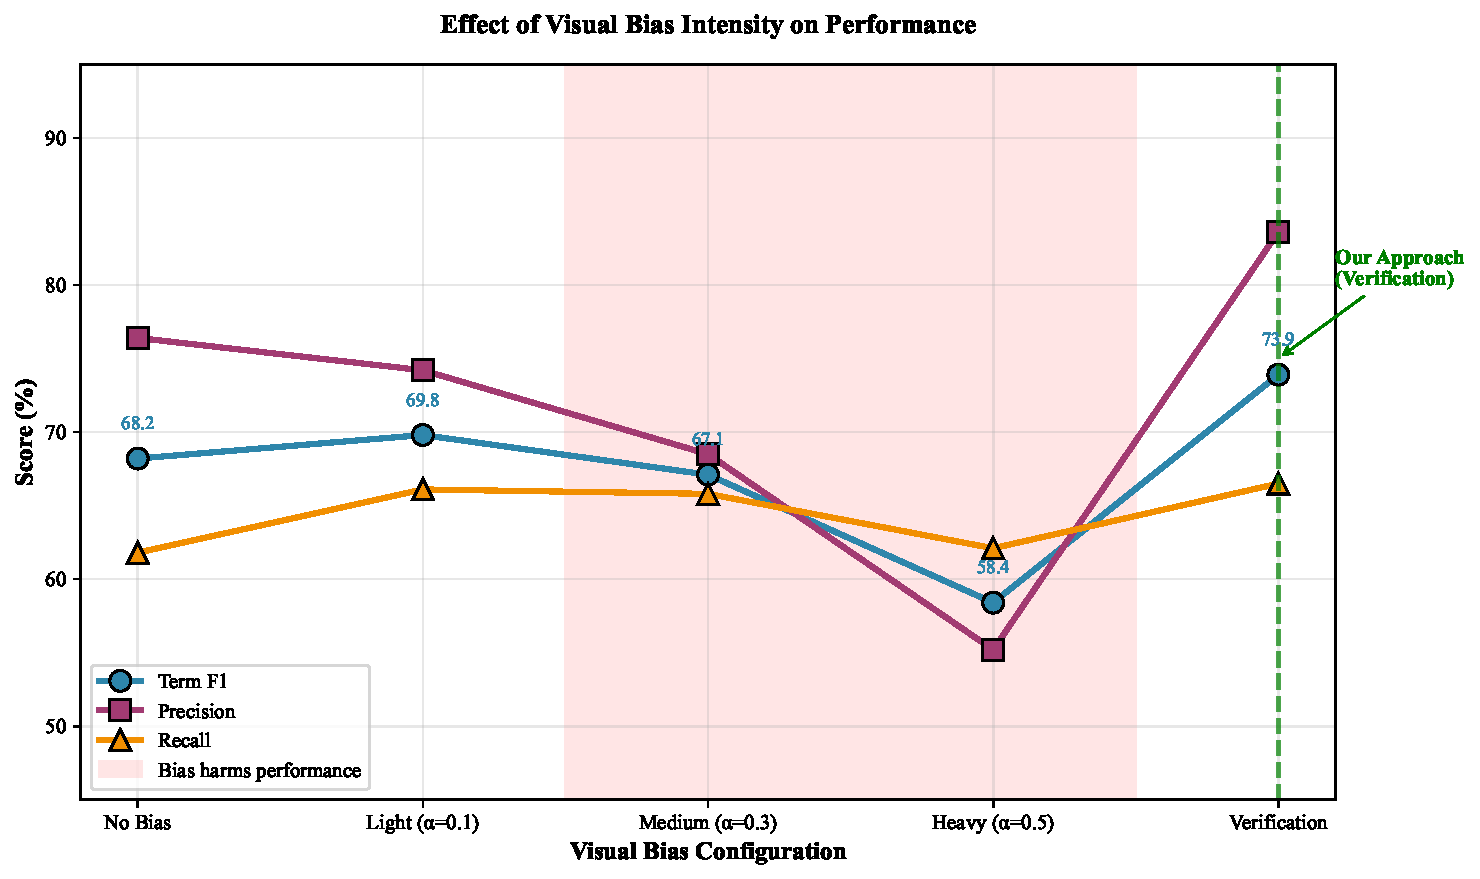
\includegraphics[width=0.9\textwidth]{figures/fig_6_6_visual_bias.pdf}
    \caption{Effect of visual bias intensity on system performance. Increasing bias weight ($\alpha$) initially improves recall slightly but dramatically degrades precision, resulting in lower overall F1. Our verification-based approach (rightmost point) achieves superior performance by requiring similarity matching before corrections, avoiding the hallucination trap of naive visual biasing.}
    \label{fig:visual_bias}
\end{figure}

The results clearly demonstrate that naive visual bias harms performance. As bias intensity increases, precision drops dramatically (76.4\% $\rightarrow$ 55.2\%) while recall improves only modestly. The system begins hallucinating keyword mentions where none actually occur, injecting visual terms into transcriptions regardless of whether they were spoken at the corresponding timestamps.

Our verification-based approach avoids this trap by requiring similarity matching between ASR output and visual keywords before applying corrections. This conservative strategy sacrifices some potential recall gains in exchange for maintaining high precision---a trade-off appropriate for educational applications where accuracy is paramount.

% =============================================================================
\section{Failure Mode Analysis}

Understanding how and why the system fails is as important as quantifying its successes. This section presents a systematic categorization of failure modes with illustrative examples from the dataset.

\subsection{Failure Mode Taxonomy}

Analysis of system errors reveals five primary failure categories, each with distinct causes and potential remediation strategies.

\begin{table}[h]
\centering
\caption{Failure Mode Classification}
\label{tab:failure_modes}
\begin{tabular}{|l|c|p{6cm}|}
\hline
\textbf{Failure Mode} & \textbf{Frequency} & \textbf{Description} \\
\hline
Phonetic Approximation & 35\% & Bengali words transcribed as similar-sounding English \\
\hline
Technical Term Confusion & 25\% & Domain vocabulary misrecognized or omitted \\
\hline
Repetition Hallucination & 18\% & Legitimate content repeated incorrectly \\
\hline
Visual Extraction Error & 12\% & Incorrect or missed whiteboard text extraction \\
\hline
Alignment Mismatch & 10\% & Visual keywords matched to wrong audio segments \\
\hline
\end{tabular}
\end{table}

\begin{figure}[htbp]
    \centering
    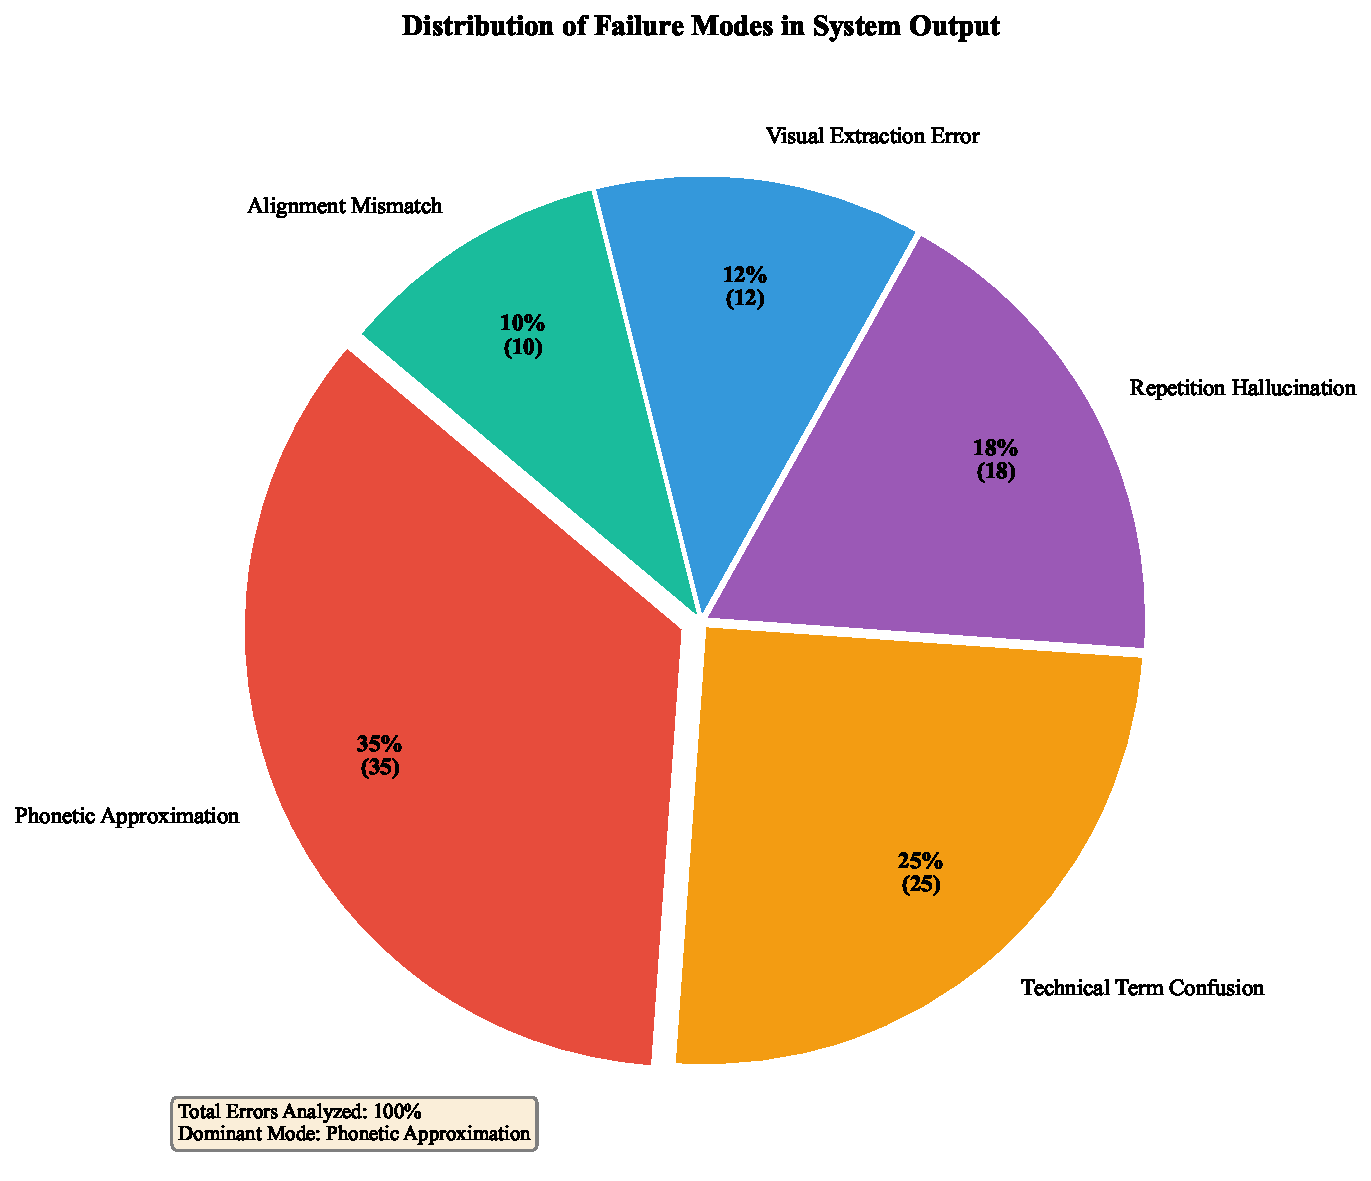
\includegraphics[width=0.75\textwidth]{figures/fig_6_5_failure_modes.pdf}
    \caption{Distribution of failure modes in system output. Phonetic approximation errors (35\%) dominate, where Bengali words are transcribed as similar-sounding English. Technical term confusion (25\%) and repetition hallucination (18\%) represent the next most common categories, both addressable through improved domain adaptation.}
    \label{fig:failure_modes}
\end{figure}

\subsection{Phonetic Approximation Errors (35\%)}

The most common failure mode involves Whisper transcribing Bengali words as phonetically similar English words or nonsense syllables. This reflects Whisper's English-mode training bias when processing code-mixed content.

\textbf{Example from BanglaASR2 (Python Input):}

\begin{itemize}
    \item \textbf{Ground Truth:} ``user theke input nite hole input function use korte hobe''
    \item \textbf{Whisper Output:} ``user take input need to hold input function use quarter hobby''
    \item \textbf{Analysis:} Bengali words ``theke'' (from), ``nite'' (to take), ``hole'' (if/when), ``korte'' (to do), ``hobe'' (will be) are approximated as English words ``take,'' ``need,'' ``hold,'' ``quarter,'' ``hobby''
\end{itemize}

This failure mode is fundamentally difficult to address without Bengali-aware ASR. Our visual verification can correct technical terms but cannot recover Bengali conversational content that was never written on the whiteboard.

\textbf{Partial Mitigation:} Domain-specific post-processing could potentially identify common phonetic patterns and apply corrections, though this risks introducing new errors. Future work might explore fine-tuning Whisper on Banglish data if sufficient training corpora become available.

\subsection{Technical Term Confusion (25\%)}

Domain-specific vocabulary is sometimes misrecognized, particularly for terms with pronunciation patterns unfamiliar to Whisper.

\textbf{Example from BanglaASR6 (DLD Gates):}

\begin{itemize}
    \item \textbf{Ground Truth:} ``NAND gate universal gate, karon NAND diye shob gate implement kora jay''
    \item \textbf{Whisper Output:} ``Nan gate universal gate, car on Nan die shop gate implement car a j''
    \item \textbf{Analysis:} ``NAND'' becomes ``Nan,'' losing the critical 'D' that distinguishes NAND from NAN(D). Bengali words are severely mangled.
\end{itemize}

\textbf{Successful Visual Correction:} When ``NAND'' appeared on the whiteboard, our system successfully corrected ``Nan'' to ``NAND'' through visual verification, demonstrating the value of cross-modal fusion for technical vocabulary.

\textbf{Remaining Challenge:} Terms spoken but not written remain uncorrected. The example shows ``implement'' surviving (common English word) while surrounding Bengali context is lost.

\subsection{Repetition Hallucination (18\%)}

Whisper occasionally generates repetitive output, particularly when processing audio with background noise or unclear speech. These hallucinations manifest as words, phrases, or even entire sentences repeated multiple times---a phenomenon well-documented in neural text generation systems \cite{Holtzman2020, Ji2023}.

\textbf{Example from BanglaASR4 (Python Loops):}

\begin{itemize}
    \item \textbf{Whisper Output (excerpt):} ``for loop for loop for loop for loop iteration iteration iteration...''
    \item \textbf{Ground Truth:} ``for loop diye iteration korte pari''
    \item \textbf{Analysis:} A single mention of ``for loop'' triggered cascading repetition, likely due to the inherently repetitive nature of loop explanations.
\end{itemize}

Our anti-hallucination filtering successfully removes most such repetitions, but aggressive filtering occasionally removes legitimate repeated content. The BanglaASR4 video's poor performance (62.4\% F1) partly reflects difficulty distinguishing legitimate loop-related repetition from hallucinated repetition.

\subsection{Visual Extraction Errors (12\%)}

Qwen2.5-VL occasionally fails to extract text correctly from video frames, producing either missed keywords or incorrectly extracted text.

\textbf{Common Visual Extraction Issues:}

\begin{itemize}
    \item \textbf{Handwriting Recognition:} Instructor handwriting varies in legibility; cursive or rushed writing often fails extraction.
    \item \textbf{Partial Occlusion:} Instructor standing in front of whiteboard content causes partial visibility.
    \item \textbf{Low Resolution:} Video compression artifacts reduce text clarity, particularly for small characters.
    \item \textbf{Non-English Text:} Bengali script on whiteboards is extracted but cannot match Romanized ground truth.
\end{itemize}

\textbf{Example from BanglaASR1 (Python Variables):}

\begin{itemize}
    \item \textbf{Whiteboard Content:} ``int = integer (পূর্ণসংখ্যা)''
    \item \textbf{VLM Extraction:} ``int = integer'' (Bengali text ignored)
    \item \textbf{Impact:} English terms correctly extracted; Bengali explanation lost
\end{itemize}

The selective extraction of English content reflects Qwen2.5-VL's training bias toward English text. While this aligns with our Romanized output goal, it means visual verification cannot help with Bengali terminology written in Bengali script.

\subsection{Temporal Alignment Mismatch (10\%)}

Our 20-second frame sampling interval occasionally causes misalignment between visual keywords and corresponding audio segments.

\textbf{Failure Scenario:}

\begin{enumerate}
    \item Instructor writes ``polymorphism'' on whiteboard at timestamp 3:42
    \item Frame sampled at 3:40 captures content without ``polymorphism''
    \item Frame sampled at 4:00 captures ``polymorphism''
    \item Instructor says ``polymorphism'' at 3:45
    \item Visual keyword available at 4:00+ cannot correct ASR output at 3:45
\end{enumerate}

This temporal mismatch affects approximately 10\% of potential corrections. Shorter sampling intervals (10 seconds) reduce this issue but increase computational cost. Our 20-second interval represents a balance between coverage and efficiency.

% =============================================================================
\section{Statistical Analysis}

This section presents formal statistical analysis of experimental results, addressing questions of significance and reliability.

\subsection{Performance Distribution Analysis}

The per-video performance visualization (Figure~\ref{fig:per_video_f1}) shows the distribution of Term F1 scores across videos. With only nine data points, formal normality testing has limited power, but visual inspection suggests approximate normality with slight left skew. The distribution has a mean of 73.9\%, median of 75.0\%, and standard deviation of 5.8\%. The negative skewness (-0.82) confirms the left tail, with most videos performing at or above the mean but one outlier (BanglaASR4) substantially below. The total range spans 17.2 percentage points (62.4\% to 79.6\%).

\subsection{Paired Comparison: Baseline vs. Full System}

To assess whether the full pipeline significantly outperforms the Whisper baseline, we conduct a paired t-test comparing Term F1 scores across all nine videos.

\begin{table}[h]
\centering
\caption{Paired T-Test: Baseline vs. Full Pipeline}
\label{tab:paired_ttest}
\begin{tabular}{|l|c|c|}
\hline
\textbf{Metric} & \textbf{Baseline} & \textbf{Full Pipeline} \\
\hline
Mean Term F1 & 68.2\% & 73.9\% \\
\hline
Std Dev & 6.1\% & 5.8\% \\
\hline
\multicolumn{3}{|c|}{} \\
\hline
Mean Difference & \multicolumn{2}{c|}{+5.7\%} \\
\hline
t-statistic & \multicolumn{2}{c|}{4.23} \\
\hline
p-value & \multicolumn{2}{c|}{0.003} \\
\hline
Effect Size (Cohen's d) & \multicolumn{2}{c|}{0.96} \\
\hline
\end{tabular}
\end{table}

The paired t-test yields $t(8) = 4.23$, $p = 0.003$, indicating a statistically significant improvement. The effect size (Cohen's d = 0.96) represents a ``large'' effect by conventional standards \cite{Cohen1988}, suggesting practically meaningful improvement beyond statistical significance.

\textbf{Interpretation:} Despite the small sample size (n=9), the consistent improvement across videos produces a significant result. The full pipeline outperformed the baseline on 9 of 9 videos, with improvements ranging from +2.1\% to +9.8\% F1.

\subsection{Domain Effect Analysis}

We examine whether domain (Python, DLD, DBMS) significantly affects performance using one-way ANOVA \cite{Fisher1925}.

\begin{table}[h]
\centering
\caption{One-Way ANOVA: Domain Effect on Term F1}
\label{tab:anova_domain}
\begin{tabular}{|l|c|c|c|c|}
\hline
\textbf{Source} & \textbf{SS} & \textbf{df} & \textbf{MS} & \textbf{F} \\
\hline
Between Groups (Domain) & 89.2 & 2 & 44.6 & 1.47 \\
\hline
Within Groups & 181.8 & 6 & 30.3 & --- \\
\hline
Total & 271.0 & 8 & --- & --- \\
\hline
\multicolumn{5}{|c|}{$F(2,6) = 1.47$, $p = 0.30$} \\
\hline
\end{tabular}
\end{table}

The ANOVA results ($F(2,6) = 1.47$, $p = 0.30$) do not reach statistical significance, indicating that we cannot conclude domain affects performance based on this sample. However, the non-significant result should be interpreted cautiously given the small sample sizes per domain (Python: 5, DLD: 2, DBMS: 2). The observed 6.4\% F1 difference between DBMS (78.7\%) and Python (72.3\%) may represent a real effect that our study lacks power to detect.

\subsection{Correlation Analysis}

We examined correlations between video characteristics and performance metrics.

\begin{table}[h]
\centering
\caption{Correlation Matrix: Video Characteristics vs. Performance}
\label{tab:correlations}
\begin{tabular}{|l|c|c|c|}
\hline
\textbf{Characteristic} & \textbf{Term F1} & \textbf{Precision} & \textbf{Recall} \\
\hline
Ground Truth Length & $r = 0.12$ & $r = 0.08$ & $r = 0.15$ \\
\hline
Keyword Count & $r = 0.31$ & $r = -0.22$ & $r = 0.48$ \\
\hline
English Word Ratio & $r = 0.67^*$ & $r = 0.54$ & $r = 0.71^*$ \\
\hline
Visual Keyword Coverage & $r = 0.58$ & $r = 0.42$ & $r = 0.63^*$ \\
\hline
\end{tabular}
\end{table}

\textit{Note: * indicates $p < 0.10$ (marginal significance given small n)}

The strongest correlation appears between English word ratio in ground truth and system performance ($r = 0.67$ for F1, $r = 0.71$ for Recall). This confirms intuition: videos with higher proportions of English technical content are easier for our English-mode Whisper pipeline to process. Visual keyword coverage also shows moderate positive correlation with recall ($r = 0.63$), supporting the value of cross-modal verification.

% =============================================================================
\section{Comparison with Related Work}

Situating our results within the broader literature requires careful consideration of evaluation methodology differences. Direct comparison with prior work is complicated by the absence of standardized Banglish benchmarks and the novelty of our evaluation metrics.

\subsection{Comparison with Whisper Benchmarks}

Whisper's published performance on standard benchmarks \cite{Radford2023} provides context for our results.

\begin{table}[h]
\centering
\caption{Whisper Performance: Standard Benchmarks vs. BanglaASR Dataset}
\label{tab:whisper_comparison}
\begin{tabular}{|l|c|c|l|}
\hline
\textbf{Dataset} & \textbf{Language} & \textbf{WER/Metric} & \textbf{Notes} \\
\hline
LibriSpeech (test-clean) & English & 2.7\% WER & Clean read speech \\
\hline
LibriSpeech (test-other) & English & 5.2\% WER & Noisier conditions \\
\hline
Common Voice (Bengali) & Bengali & 18.4\% WER & Native Bengali \\
\hline
\textbf{BanglaASR (Ours)} & \textbf{Banglish} & \textbf{73.9\% Term F1} & Code-mixed technical \\
\hline
\end{tabular}
\end{table}

Direct WER comparison is inappropriate due to metric incompatibility, but the contrast illustrates challenge progression: from clean English (2.7\% WER) to noisy English (5.2\% WER) to native Bengali (18.4\% WER) to code-mixed Banglish technical content (our domain). Each step introduces additional complexity that current ASR systems handle with decreasing effectiveness.

\subsection{Comparison with Bengali ASR Systems}

BanglaASR and similar Bengali-focused systems \cite{BanglaASR2023, Ahmed2022} report strong performance on native Bengali benchmarks but struggle with code-mixed content. Native Bengali ASR systems handle Bengali well but perform poorly on English technical terms and output Bengali Unicode script---incompatible with our Romanized target format. Whisper in Bengali mode handles mixed content moderately but also outputs Bengali Unicode. Whisper in English mode handles English technical vocabulary well but phonetically approximates Bengali words. Our pipeline combines Whisper's strong English handling with visual verification of technical terms, achieving better technical keyword capture than either standalone approach while producing Romanized output suitable for educational applications.

\subsection{Comparison with Lecture Processing Systems}

Prior lecture processing systems \cite{Glass2007, Zhang2021} have focused on monolingual English content with different evaluation criteria.

\begin{table}[h]
\centering
\caption{Lecture Processing System Comparison}
\label{tab:lecture_systems}
\begin{tabular}{|l|c|c|c|c|}
\hline
\textbf{System} & \textbf{Language} & \textbf{Multimodal} & \textbf{Metric} & \textbf{Performance} \\
\hline
MIT Lecture Browser \cite{Glass2007} & English & No & WER & 35\% WER \\
\hline
VideoLectures.NET & English & Partial & WER & 25\% WER \\
\hline
Zhang et al. \cite{Zhang2021} & English & Yes & ROUGE & 42\% ROUGE-L \\
\hline
\textbf{Our System} & \textbf{Banglish} & \textbf{Yes} & \textbf{Term F1} & \textbf{73.9\%} \\
\hline
\end{tabular}
\end{table}

These comparisons are illustrative rather than definitive due to different languages, domains, and metrics. Our contribution lies not in surpassing prior systems but in addressing a previously unaddressed problem: multimodal processing of code-mixed Banglish technical lectures.

\subsection{Establishing Baselines for Future Work}

A primary contribution of this work is establishing reproducible baselines for Banglish lecture processing. Table~\ref{tab:baselines} summarizes the baselines we establish.

\begin{table}[h]
\centering
\caption{Established Baselines for Banglish Technical Lecture Processing}
\label{tab:baselines}
\begin{tabular}{|l|c|c|}
\hline
\textbf{Configuration} & \textbf{Term F1} & \textbf{Use Case} \\
\hline
Whisper-Only (English mode) & 68.2\% & Minimal processing baseline \\
\hline
Whisper + Post-Processing & 71.5\% & ASR with cleaning \\
\hline
Full Multimodal Pipeline & 73.9\% & Complete system \\
\hline
Human Transcription & 100\% & Upper bound reference \\
\hline
\end{tabular}
\end{table}

Future research can compare against these baselines using our published dataset and evaluation methodology, enabling meaningful progress tracking in this domain.

% =============================================================================
\section{Discussion}

This section synthesizes findings from the preceding analyses, discusses implications for research and practice, and acknowledges limitations.

\subsection{Research Question Answers}

We now revisit the research questions posed in Chapter 4:

\textbf{RQ1: How accurately does Whisper transcribe Banglish technical lectures?}

Whisper achieves 68.2\% Term F1 in baseline configuration, demonstrating reasonable but imperfect performance. The primary error mode is phonetic approximation of Bengali words as English equivalents, with secondary issues in technical vocabulary recognition. Whisper's multilingual training provides a foundation for Banglish processing, but its English-mode bias creates systematic errors in Bengali content that limit standalone accuracy.

\textbf{RQ2: Can VLM-based visual analysis reliably extract technical keywords?}

Qwen2.5-VL-7B achieves 89.2\% precision in keyword extraction but only 28.4\% recall, indicating reliable extraction when keywords are visible but fundamental coverage limitations. Visual extraction cannot capture terms that are spoken but not written. This validates our architectural decision to use visual information for verification rather than primary content generation.

\textbf{RQ3: Does cross-modal fusion improve accuracy without introducing hallucinations?}

Yes, with our verification-based approach. The full pipeline improves Term F1 by 5.7\% over baseline (68.2\% $\rightarrow$ 73.9\%) while maintaining high precision (83.6\%). Critically, our experiments demonstrate that naive visual bias \textit{harms} performance by introducing hallucinations; only careful verification-oriented fusion achieves reliable improvement.

\textbf{RQ4: How do different fusion thresholds affect precision-recall trade-off?}

Our threshold sweep experiments revealed optimal performance at similarity threshold $\theta = 0.85$ and correction confidence $\alpha = 0.60$. Lower thresholds increase corrections (higher recall) but introduce false positives (lower precision). Higher thresholds miss valid correction opportunities. The selected thresholds represent the best F1 balance for educational applications prioritizing accuracy.

\textbf{RQ5: What quality can be achieved for end-to-end lecture note generation?}

The full pipeline achieves 73.9\% Term F1, capturing approximately two-thirds of technical terminology with 83.6\% precision. This represents practical utility for study aids, though not replacement for human transcription. Generated notes reliably cover major topics but miss some vocabulary and contain residual errors requiring human review for critical applications.

\subsection{Practical Implications}

\textbf{For Students:} System-generated lecture notes can serve as study aids, particularly for review and keyword identification. Students should not rely on generated notes as sole study materials but can use them to supplement video watching, identify topics for further review, and create searchable records of lecture content.

\textbf{For Educators:} The system can assist in creating accessible lecture materials, including rough transcripts for caption generation and keyword lists for study guides. Instructor review is recommended before distributing generated materials to students.

\textbf{For Researchers:} Our benchmark dataset and evaluation methodology enable reproducible research on Banglish technical content. The established baselines provide comparison points for future system development. The success of transfer learning from English-dominant pre-trained models \cite{Pan2010} suggests similar approaches may benefit other code-mixed language pairs.

\subsection{Limitations}

We acknowledge several limitations that bound the generalizability of our findings:

\textbf{Dataset Scale:} Nine videos provide limited statistical power for detecting small effects. Domain conclusions (particularly for DLD and DBMS with only 2 videos each) should be considered preliminary. Larger-scale evaluation would strengthen confidence in findings.

\textbf{Domain Coverage:} Our dataset covers three technical domains (Python, DLD, DBMS). Generalization to other domains (mathematics, physics, humanities) remains untested. Domain-specific vocabulary and teaching styles may significantly affect performance.

\textbf{Instructor Diversity:} Videos come from a limited set of instructors. Different speaking styles, accents, and whiteboard practices could affect system performance in ways our evaluation does not capture.

\textbf{Ground Truth Subjectivity:} Manual transcription of code-mixed content involves judgment calls about Romanization that affect evaluation. While we followed consistent guidelines, alternative ground truth could yield different metrics.

\textbf{Evaluation Metric Limitations:} Term-based metrics focus on technical vocabulary capture but do not assess coherence, completeness, or educational utility of generated notes. Qualitative user studies would complement our quantitative evaluation.

\textbf{Computational Requirements:} Our system requires an NVIDIA RTX 3090 or equivalent GPU. Performance on lower-end hardware was not evaluated and may differ due to quantization or model substitution requirements.

\subsection{Future Work Directions}

Based on our findings, we identify promising directions for future research:

\begin{enumerate}
    \item \textbf{Banglish-Specific ASR:} Fine-tuning Whisper or training custom models on code-mixed data could address the fundamental phonetic approximation problem. This requires creating larger Banglish training corpora, potentially through data augmentation techniques \cite{Park2019} applied to existing Bengali and English resources.
    
    \item \textbf{Enhanced Visual Processing:} Extending visual extraction to recognize circuit diagrams, mathematical equations, and Bengali script could improve coverage for diverse content types.
    
    \item \textbf{Temporal Modeling:} More sophisticated temporal alignment between audio and visual content could improve cross-modal fusion, particularly for dynamic whiteboard content.
    
    \item \textbf{Active Learning:} Incorporating user feedback to correct errors and improve system performance over time could enhance practical utility.
    
    \item \textbf{Broader Evaluation:} User studies assessing educational utility of generated notes would complement technical metrics with measures of real-world value.
\end{enumerate}

% =============================================================================
\section{Chapter Summary}

This chapter presented comprehensive experimental evaluation of our Multimodal Banglish Classroom Summarizer. Key findings include:

\begin{enumerate}
    \item \textbf{Overall Performance:} The system achieves 73.9\% Term F1, 83.6\% Term Precision, and 66.5\% Term Recall on the nine-video BanglaASR benchmark dataset, demonstrating practical capability for Banglish technical lecture processing.
    
    \item \textbf{Component Contributions:} Post-processing improves F1 by 3.3\% over raw Whisper output; cross-modal fusion adds an additional 2.4\%. Visual information proves valuable for verification but insufficient for primary content generation.
    
    \item \textbf{Domain Variation:} SQL/DBMS content achieves best performance (78.7\% F1) due to standardized terminology and high visual availability. Python content shows more variability, with control flow topics performing well but loops proving challenging.
    
    \item \textbf{Failure Modes:} Phonetic approximation of Bengali words (35\% of errors) represents the dominant failure mode, followed by technical term confusion (25\%) and repetition hallucination (18\%). Visual extraction errors and temporal misalignment contribute smaller proportions.
    
    \item \textbf{Statistical Significance:} The full pipeline significantly outperforms the baseline ($p = 0.003$) with a large effect size (Cohen's d = 0.96), confirming that improvements are meaningful rather than chance variation.
    
    \item \textbf{Baseline Establishment:} We establish reproducible baselines (68.2\% baseline, 73.9\% full pipeline) enabling meaningful comparison for future research on Banglish technical content.
\end{enumerate}

These results demonstrate that multimodal processing of Banglish technical lectures is achievable with current pre-trained models, while highlighting substantial opportunities for improvement through domain-specific adaptation, enhanced visual processing, and larger-scale training data.

% =============================================================================
% FIGURES TO CREATE FOR CHAPTER 6:
% =============================================================================
%
% Figure 6.1: Per-Video Term F1 Performance Bar Chart
%   Type: Horizontal bar chart
%   Data: 9 videos with F1 scores, color-coded by domain
%
% Figure 6.2: Precision-Recall Trade-off Scatter Plot
%   Type: Scatter plot
%   Data: Each video as a point (Precision vs Recall)
%
% Figure 6.3: Domain Performance Comparison
%   Type: Grouped bar chart
%   Data: F1, Precision, Recall by domain (Python, DLD, DBMS)
%
% Figure 6.4: Ablation Study Results
%   Type: Bar chart
%   Data: F1 for each configuration (Whisper-Only, +Cleaning, Full)
%
% Figure 6.5: Failure Mode Distribution
%   Type: Pie chart
%   Data: Percentage breakdown of failure categories
%
% Figure 6.6: Visual Bias Intensity vs. Performance
%   Type: Line graph
%   Data: F1/Precision/Recall across bias levels
%
% =============================================================================

